Soit $\widehat{ADM} = \phi$ et $\widehat{MDC}=\phi'$. On a $\phi + \phi' = 90^\circ$.

Donc $\widehat{MNC} = 180^\circ - 90^\circ - \widehat{BMN} = \phi'$.

Donc, comme $\widehat{DNC} = \widehat{CDN} = \phi'$, on a : $CD = CN$.

Comme $\widehat{ADC} = \widehat{AHD} = 90^\circ$, on a $CD^2=CH\cdot CA$ et $AD^2 = AH\cdot AC$. Il suit : $CN^2 = CH\cdot CA ~~(1)$ et $AM^2 = AH\cdot AC~~(2)$

D'après $(2)$ : $\widehat{AHM} = \widehat{AMC}$ puis $\widehat{CHM} = \widehat{CMB}~~(3)$.

D'après $(1)$ : $\widehat{CHN} = \widehat{CNA}~~(4)$.

En faisant $(4)-(3)$ : $\widehat{NHM} = \widehat{CNA} - \widehat{CMB}$.

Il reste à montrer : $\widehat{MCK} = \widehat{CNA} - \widehat{CMB}$.

Soit $J=AB\cap CK$. Comme $\widehat{JBN} = \widehat{JKN} = 90^\circ$, $J, B, K, N$ sont cocycliques, donc
\begin{align*}
\widehat{MCK}
& = \widehat{MCJ} \\
& = 180^\circ - \widehat{MJC} - \widehat{CMB} \\
& = 180^\circ - \widehat{KJB} - \widehat{CMB} \\
& = \widehat{KNB} - \widehat{CMB} \\
& = \widehat{CNA} - \widehat{CMB}
\end{align*}

\begin{center}
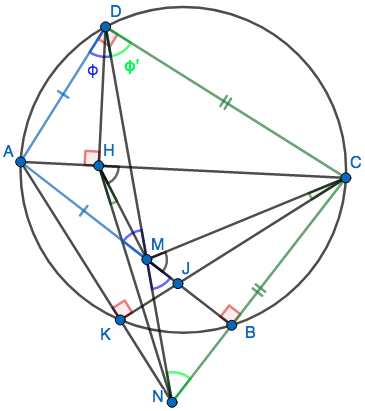
\includegraphics{sol-130.png}
\end{center}